%\documentclass[10pt,handout]{beamer}
\documentclass[10pt]{beamer}
\usepackage[ngerman]{babel}
\usepackage[utf8]{inputenc}
\usepackage{amsmath}
\usepackage{amssymb}
\usepackage{listings} 
\usepackage{mathtools}
\usepackage{ulem}
\usepackage{hyperref}
\usepackage{eurosym}
\usetheme{Boadilla}

\parskip 10pt
\lstset{language=Python, tabsize=4, basicstyle=\footnotesize, showstringspaces=false,mathescape=true}  
\begin{document}
\title{ASCII, Unicode, UTF-8}   
\author{Informatik} 
\date{ } 

\frame{\titlepage} 

%-------------
\begin{frame}[fragile]
Ein Computer speichert Zahlen. Um mit Zeichen umgehen zu können, wird über
eine Zeichensatztabelle (Codepage) jedem Zeichen eine Zahl zugeordnet.
Der \textbf{ASCII-Code} (American Standard Code for Information Interchange) sieht in seiner ursprünglichen Version 7 Bits zur Codierung von Zeichen vor. Damit lassen sich $2^7 = 128$ Zeichen darstellen.  

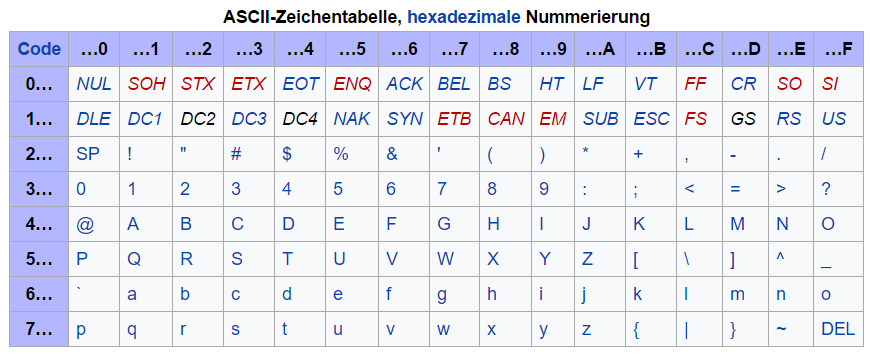
\includegraphics[scale=0.6]{bild3.png} 

\end{frame}

\begin{frame}[fragile]
ISO-8859-1 ist eine Erweiterung des ASCII-Codes auf 8 bit und reicht für die meisten westeuropäischen Sprachen aus. Es fehlt aber das Eurozeichen und einige französische Zeichen.

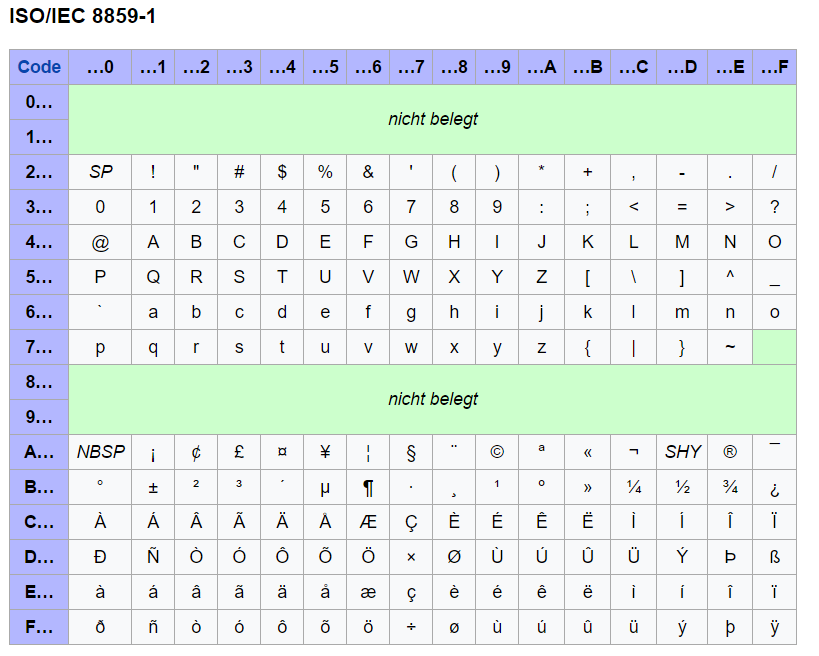
\includegraphics[scale=0.5]{bild1.png}

\end{frame}


\begin{frame}[fragile]
\textbf{Unicode} ist ein internationaler Standard, der jedem Schriftzeichen aller bekannter Sprachen einen eindeutige Zahl zuordnet (Code Point).

\begin{tabular}{c c c c}
A & $\rightarrow$ & 65 \\
a &  $\rightarrow$ & 97 \\
ß &  $\rightarrow$ & 223 \\
\EUR{} & $\rightarrow$ & 8364 \\
\end{tabular}

\textbf{UTF-8} (1992) ist die am weitesten verbreitete Kodierung für Unicode-Zeichen.
\end{frame}

\begin{frame}[fragile]
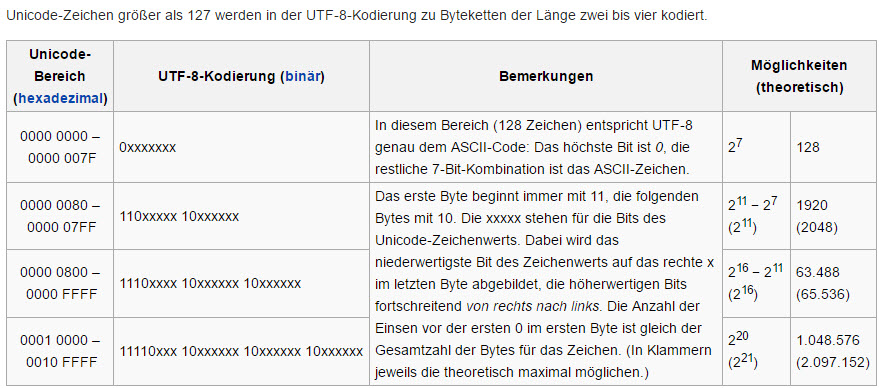
\includegraphics[scale=0.65]{bild3.jpg}

\end{frame}

\begin{frame}[fragile]
Beispiel: Die UTF-8 Codierung von \EUR{}. \\ 
Code Point (dezimal) = 8364 \\  
Code Point (hex) =  20AC  (zur Codierung werden 3 Bytes benötigt) \\  
Code Point (binär) =  0010 0000 1010 1100 \\  
Aufteilung der bits in die 3 Bytes  : \\ 
\texttt{1110xxxx 10xxxxxx 10xxxxxx} \\ 
\texttt{11100010 10000010 10101100} \\ 
E2 82 AC   ist die Codierung des Eurozeichens.
\end{frame}

\begin{frame}[fragile]
In Python ist ein String-Objekt eine Folge von Zeichen in Unicode. Die Funktionen \texttt{chr} und \texttt{ord}
wandeln den Unicode-Codepoint in das Zeichen um und umgekehrt. 

Die Methode \texttt{encode('utf8')} gibt die UTF-8 Codierung des Zeichens als Bytefolge zurück. 

\begin{lstlisting}  

>>> '\u20ac'
'$\text{\EUR{}}$'
>>> chr(8364)
'$\text{\EUR{}}$'
>>> chr(8364).encode('utf8')
b'\xe2\x82\xac'
>>> 
\end{lstlisting} 
\end{frame}


\begin{frame}[fragile]
Ein Texteditor soll folgenden Speicherbereich darstellen:

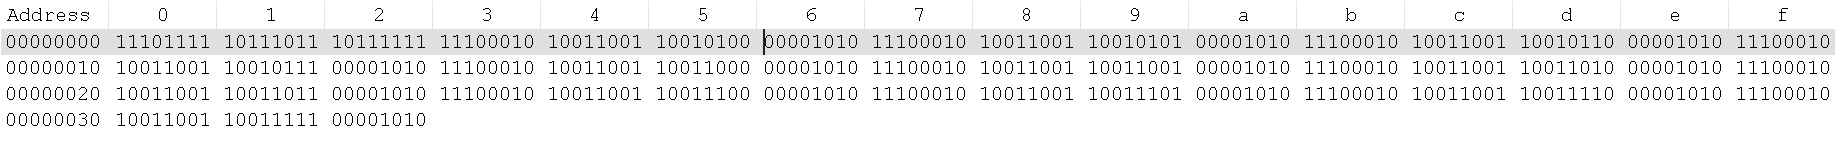
\includegraphics[scale=0.3]{bild4.png} \pause

Derselbe Speicherbereich hexadezimal:

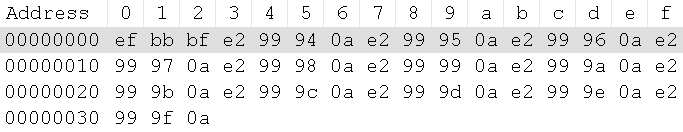
\includegraphics[scale=0.5]{bild5.png}  

Die Bytefolge \texttt{EF BB BF} heißt \textbf{Byte Order Mark (BOM)} und gibt den Editor einen Hinweis darauf, dass
eine UTF-8 Kodierung vorliegt.   \\
\texttt{0A} ist die ASCII (und UTF-8) Codierung für den Zeilenvorschub. \pause

\texttt{E2 99 94} ist die UTF-8 Codierung des hexadezimalen Codepoints \texttt{2654} 


\end{frame}

\begin{frame}[fragile]
Darstellung der Bit-Folge mit dem Font \texttt{Lucida Sans Unicode}.


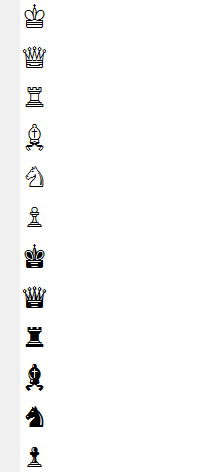
\includegraphics[scale=0.5]{bild7.png} 

\end{frame}

 \end{document}
